\documentclass[11pt]{article}
\usepackage[margin=1in]{geometry}
\usepackage{amsmath,amssymb,amsthm}
\usepackage{graphicx}
\usepackage{booktabs}
\usepackage[colorlinks=true,linkcolor=blue,citecolor=blue,urlcolor=blue]{hyperref}

\theoremstyle{plain}
\newtheorem{proposition}{Proposition}
\newtheorem{corollary}{Corollary}
\theoremstyle{definition}
\newtheorem{remark}{Remark}

\title{\bf Topological Collapse and Asymmetric Divergence\\
of Carmichael Pseudoprimes on the $6N$ Skeleton%
\thanks{Code and measured data: \url{https://github.com/Ruqing1963/6N-carmichael-collapse} (Part XXXVI).}}
\author{Ruqing Chen\\
\small GUT Geoservice Inc., Montreal, Quebec, Canada\\
\small \texttt{ruqing@hotmail.com}}
\date{June 9, 2026}

\begin{document}
\maketitle

\begin{abstract}
On the $6N$ skeleton every integer coprime to $6$ sits on a wing: the right wing $6N{+}1$
($\equiv1\bmod6$) or the left wing $6N{-}1$ ($\equiv5\bmod6$). We read the Carmichael numbers
through this geometry. Korselt's criterion forces a sharp, elementary structure that we state and
verify: \emph{(i)} a one-way semipermeable membrane---every Carmichael number on the left wing has
\emph{all} of its prime factors on the left wing (and is not divisible by $3$); \emph{(ii)} a
parity law---a Carmichael number coprime to $6$ lies on the left wing iff it has an odd number of
left-wing prime factors; and \emph{(iii)} a unified barrier---whenever $3\nmid(n-1)$ no right-wing
prime can divide $n$, which fuses the left wing with the off-skeleton residue-$3$ numbers (a
residue-$3$ Carmichael number is exactly a $3$ glued to a pure-left core). Enumerating all $1547$
Carmichael numbers up to $10^{10}$, all three laws hold with \emph{zero} violations. The geometric
consequence is a violent asymmetry: the right-to-left ratio $R(X)=\#\{\text{right}\}/\#\{\text{left}\}$
climbs monotonically from $5.0$ at $X=10^{4}$ to $88.8$ at $X=10^{10}$, a collapse of the left-wing
population across seven decades. The same monochromatic suppression acts \emph{inside} the right wing:
the pure-right family is overtaken by the mixed family, the internal ratio
$M(X)=\#\{\text{pure-right}\}/\#\{\text{mixed}\}$ crossing unity between $10^{7}$ and $10^{8}$. We trace
the mechanism to a single structural fact---single-colour cores require all factors in one wing, while
the mean number of prime factors $\bar k(X)$ grows ($3.00\to4.23$)---but we are explicit that the two
single-colour basins are \emph{not} symmetric: pure-right decays about $2.6$ times more slowly than the
left wing in the $\log$-exponent, because right-wing primes have smooth ($6\mid p-1$) and left-wing
primes rough ($3\nmid p-1$) predecessors. We claim no unified thermodynamic law: there is no single
decay exponent, and the divergence \emph{rate} is itself not identifiable---a power of $\log X$, a small
power of $X$, and a stretched exponential fit equally well, and Poisson sparsity plus the deep
pre-asymptotic character of Carmichael statistics put the asymptotic law beyond any reachable window.
What is unified is \emph{algebraic} (the single barrier of law \emph{(iii)}), not thermodynamic; the
structural laws and the asymmetric-collapse phenomenon are firm, the asymptotic divergence law is, by
construction, beyond reach.
\end{abstract}

\section{Introduction}
A Carmichael number is a composite $n$ for which $a^{n}\equiv a\pmod n$ for every integer $a$; by
Korselt's criterion \cite{Korselt} these are exactly the squarefree $n$ with at least three prime
factors such that $p-1\mid n-1$ for every prime $p\mid n$. They are infinite in number
\cite{AGP}, but their finer distribution---the growth of $C(x)=\#\{\text{Carmichael}\le x\}$ and the
internal correlations among their prime factors---remains, in Erd\H{o}s's heuristic \cite{Erdos} and
in Pinch's tabulations \cite{Pinch}, only partly understood.

The present series reads arithmetic objects through the $6N$ skeleton, on which every prime $>3$ lies
on a fault line $6N\pm1$. Here we ask what Korselt's criterion looks like in that geometry. The answer
is an elementary but unusually rigid structure, and a measured macroscopic consequence. We make no
claim that the structural facts are new as mathematics---they follow in a few lines from Korselt---only
that their statement in the wing coordinates is clean, and that the resulting population asymmetry, and
its honest non-identifiability, are worth recording.

\section{The structural laws}
Write a prime $p>3$ as \emph{right} if $p\equiv1\pmod6$ and \emph{left} if $p\equiv5\pmod6$. On the
units $(\mathbb Z/6)^{\times}=\{1,5\}\cong\{\pm1\}$, right primes carry the residue $+1$ and left
primes the residue $-1$.

\begin{proposition}[The semipermeable membrane]\label{prop:membrane}
Let $n$ be a Carmichael number with $n\equiv5\pmod6$ (the left wing). Then $3\nmid n$ and every prime
factor of $n$ satisfies $p\equiv5\pmod6$. No right-wing prime, and no factor of $3$, can occur.
\end{proposition}

\begin{proof}
$n\equiv5\pmod6$ gives $n$ odd and $3\nmid n$, so $n$ is coprime to $6$ and every prime factor is
$\equiv1$ or $\equiv5\pmod6$. Suppose $p\mid n$ with $p\equiv1\pmod6$. Then $6\mid p-1$. By Korselt
$p-1\mid n-1$, hence $6\mid n-1$. But $n\equiv5\pmod6$ gives $n-1\equiv4\pmod6$, so $6\nmid n-1$---a
contradiction. Thus no factor is $\equiv1\pmod6$, and all factors are $\equiv5\pmod6$.
\end{proof}

\begin{proposition}[The parity law]\label{prop:parity}
Let $n$ be a Carmichael number coprime to $6$, with $\ell$ prime factors $\equiv5\pmod6$ (counted with
the multiplicity $1$, as $n$ is squarefree). Then $n\equiv(-1)^{\ell}\pmod6$. Equivalently: $n$ is on
the right wing iff $\ell$ is even, and on the left wing iff $\ell$ is odd.
\end{proposition}

\begin{proof}
Modulo $6$ the residue of a product of units is the product of residues; right factors contribute $+1$
and left factors $-1$, so $n\equiv(+1)^{\#\text{right}}(-1)^{\ell}\equiv(-1)^{\ell}\pmod6$.
\end{proof}

\begin{corollary}\label{cor:left}
A left-wing Carmichael number is a product of an \emph{odd} number ($\ge3$) of distinct primes, all
$\equiv5\pmod6$. The left wing is the single monochromatic, odd-length family; the right wing
collects everything else---the all-right products, and all mixed products with an even number of left
factors.
\end{corollary}

The membrane of Proposition~\ref{prop:membrane} is not special to the left wing. Its true cause is the
divisibility of $n-1$ by $3$, and stating it that way unifies the left wing with the third class---the
Carmichael numbers divisible by $3$, which leave the skeleton at residue $3\pmod6$ (e.g.\
$561=3\cdot11\cdot17$).

\begin{proposition}[The unified barrier]\label{prop:barrier}
Let $n$ be a Carmichael number with $3\nmid(n-1)$. Then $n$ has no prime factor $\equiv1\pmod6$. Among
the residues coprime to $3$ this is exactly $n\equiv5\pmod6$ (left wing) and $n\equiv3\pmod6$
($3\mid n$); in both cases every prime factor other than a possible single $3$ is $\equiv5\pmod6$.
Consequently a residue-$3$ Carmichael number is precisely $3$ times a product of distinct primes all
$\equiv5\pmod6$---a $3$ glued to a pure-left core---while a left-wing Carmichael number is a pure-left
core alone.
\end{proposition}

\begin{proof}
Suppose $p\mid n$ with $p\equiv1\pmod6$, so $3\mid p-1$. By Korselt $p-1\mid n-1$, hence $3\mid n-1$,
against the hypothesis. So no factor is $\equiv1\pmod6$. Now $3\mid n-1$ fails exactly when
$n\not\equiv1\pmod3$, i.e.\ $n\equiv2\pmod3$ ($\Leftrightarrow n\equiv5\pmod6$, the left wing) or
$3\mid n$ ($\Leftrightarrow n\equiv3\pmod6$). In the first case $3\nmid n$, so all factors are
$\equiv5\pmod6$ (recovering Proposition~\ref{prop:membrane}); in the second, $n=3m$ with $m$ squarefree
and coprime to $3$, and the argument applied to each prime of $m$ forces every such prime to be
$\equiv5\pmod6$.
\end{proof}

\begin{remark}\label{rem:unify}
The complementary case is $3\mid n-1$, i.e.\ $n\equiv1\pmod6$ (the right wing), where $p-1\equiv0\pmod6$
is permitted and right-wing factors are admitted. So a single criterion governs all three classes: the
divisor $3$ of $n-1$ is the gate. When it is absent, every right-wing prime is barred and the factor
core is forced fully onto the left wing (with, in the residue-$3$ case, an extra $3$); when it is
present, the mixed basin opens. The ``ghost'' residue-$3$ numbers are therefore not a separate
phenomenon but the $3\mid n$ face of the same barrier.
\end{remark}

These structural facts are elementary consequences of Korselt's criterion; we claim only their clean
statement and verification, not novelty as theorems. Their force is geometric: whenever $3\nmid(n-1)$
the right wing is sealed off and the factor core collapses to a single colour, while $3\mid(n-1)$ opens
the mixed basin.

\section{The measurement}
We enumerated \emph{all} Carmichael numbers up to $10^{10}$ by the Korselt divisor method (for each
ordered prefix of prime factors with product $M$, the final prime $r$ must satisfy $(r-1)\mid(M-1)$,
checked against $p-1\mid n-1$ for the remaining factors), recovering the known count $C(10^{10})=1547$
\cite{Pinch} exactly, with the correct factorisation of each. Across all $1547$ numbers,
Propositions~\ref{prop:membrane}, \ref{prop:parity}, and~\ref{prop:barrier} hold with \textbf{zero
violations}: every left-wing Carmichael number is monochromatically left, every right-wing Carmichael
number has an even number of left-wing factors, and every one of the $20$ residue-$3$ numbers up to
$10^{10}$ is a $3$ glued to a pure-left core (e.g.\ $561=3\cdot11\cdot17$, $62745=3\cdot5\cdot47\cdot89$).

Table~\ref{tab:Rx} reports the cumulative wing census by decade. The right-to-left ratio
$R(X)=\#\{n\le X:\,n\equiv1\}/\#\{n\le X:\,n\equiv5\}$ rises monotonically from $5.0$ to $88.8$.
(The residue-$3$ class, governed by Proposition~\ref{prop:barrier}, is small---$20$ numbers up to
$10^{10}$---and is excluded from the wing ratio.)

\begin{table}[h]
\centering
\begin{tabular}{rrrrrr}
\toprule
$\log_{10}X$ & $C(X)$ & right & left & $R(X)$ & $\bar k(X)$\\
\midrule
4  & 7    & 5    & 1  & 5.00  & 3.00\\
5  & 16   & 13   & 1  & 13.00 & 3.25\\
6  & 43   & 38   & 2  & 19.00 & 3.49\\
7  & 105  & 98   & 4  & 24.50 & 3.58\\
8  & 255  & 243  & 6  & 40.50 & 3.78\\
9  & 646  & 623  & 12 & 51.92 & 4.00\\
10 & 1547 & 1510 & 17 & 88.82 & 4.23\\
\bottomrule
\end{tabular}
\caption{Cumulative wing census of Carmichael numbers. $R(X)$ is the right/left ratio; $\bar k(X)$ is
the mean number of prime factors. The left-wing population collapses relative to the right as $X$
grows.}
\label{tab:Rx}
\end{table}

\begin{figure}[h]
\centering
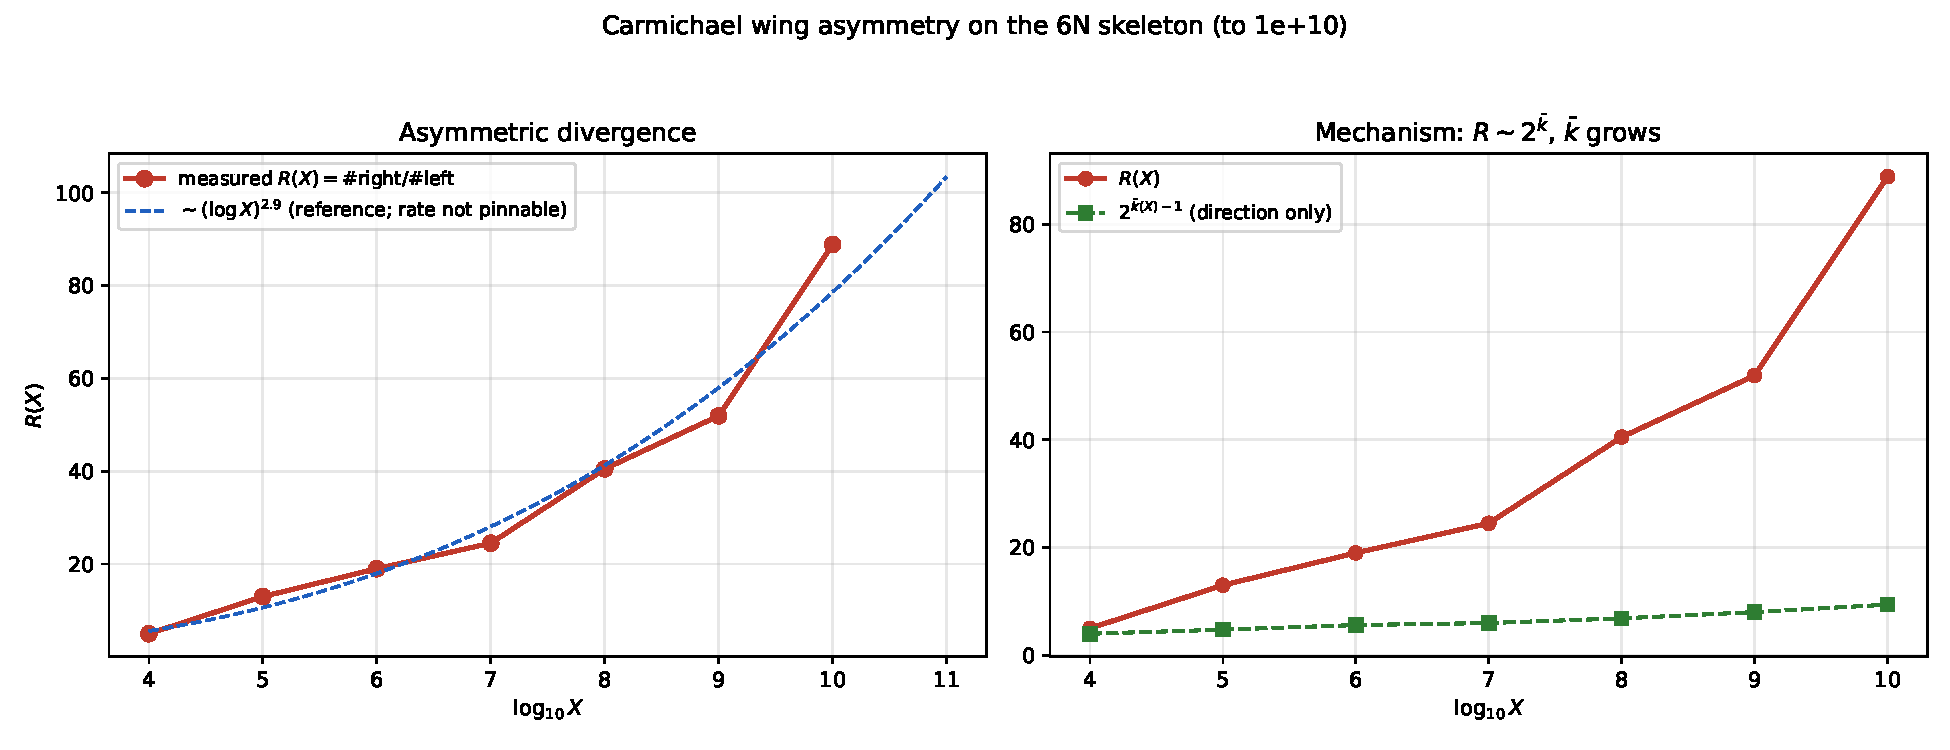
\includegraphics[width=\textwidth]{carmichael_Rx.pdf}
\caption{(Left) The measured asymmetric divergence $R(X)$ over seven decades, with a best-fitting power
of $\log X$ drawn for reference only---the rate is not identifiable (\S\ref{sec:ledger}). (Right) The mechanism:
$R(X)$ tracks the growth of the mean prime-factor count $\bar k(X)$ through the monochromatic
suppression $\sim2^{-\bar k}$; the curve $2^{\bar k-1}$ captures the direction but undershoots the
measured magnitude, because the right wing additionally absorbs the pure-right and even-mixed
families.}
\label{fig:Rx}
\end{figure}

\section{Mechanism: monochromatic suppression under a growing factor count}
By Corollary~\ref{cor:left} a left-wing Carmichael number must be \emph{monochromatic}: all of its
$k$ prime factors must fall on the left wing, with $k$ odd. For a Carmichael number with $k$ factors,
the heuristic chance that all $k$ are left-wing is of order $2^{-k}$ (the two wings carry primes of
nearly equal density). The mean number of prime factors of Carmichael numbers grows with scale---we
measure $\bar k(X)$ rising from $3.00$ to $4.23$ across the range (Table~\ref{tab:Rx})---so the
monochromatic condition becomes exponentially rarer, and the left wing is squeezed.

This is the whole of the picture, and it is only directional. The naive estimate $R\sim2^{\bar k}$
rises far more slowly than the data (Fig.~\ref{fig:Rx}, right): $2^{\bar k-1}$ runs from $4$ to $9.4$
while $R$ runs from $5$ to $89$. The shortfall is structural---the right wing is not merely
``not-all-left'' but also harvests the entire all-right family and every even-length mixed product---so
$R$ outruns $2^{\bar k}$. We name the qualitative picture a \emph{topological entropy increase}: a
low-entropy, fully ordered (single-colour) basin being absorbed into a high-entropy, mixed basin. We
use the phrase only as a mnemonic for the measured monochromatic suppression; it names a counting
asymmetry, not a dynamical law, and no entropy functional is claimed.

\section{Inside the right basin: pure-right versus mixed}
The mechanism above applies to \emph{any} single-colour core, not only the left wing. The all-right
products (every factor $\equiv1\pmod6$) are equally monochromatic, and by the same heuristic they too
should be squeezed by the mixed products as $\bar k$ grows. We test this by splitting the right wing
into its pure-right part ($\ell=0$ left factors) and its mixed part ($\ell\ge2$, necessarily even), and
tracking the internal ratio $M(X)=\#\{\text{pure-right}\}/\#\{\text{mixed}\}$.

\begin{table}[h]
\centering
\begin{tabular}{rrrr}
\toprule
$\log_{10}X$ & pure-right & mixed & $M(X)$\\
\midrule
4  & 3   & 2   & 1.50\\
5  & 8   & 5   & 1.60\\
6  & 23  & 15  & 1.53\\
7  & 53  & 45  & 1.18\\
8  & 114 & 129 & 0.88\\
9  & 254 & 369 & 0.69\\
10 & 587 & 923 & 0.64\\
\bottomrule
\end{tabular}
\caption{The right basin splits into a monochromatic pure-right family and a mixed family. The ratio
$M(X)$ crosses unity between $10^{7}$ and $10^{8}$: pure-right leads at small scale and is overtaken by
the mixed state thereafter.}
\label{tab:Mx}
\end{table}

Table~\ref{tab:Mx} confirms the prediction in direction. Pure-right leads at small scale ($M\approx1.5$),
crosses the topological transition $M=1$ between $10^{7}$ and $10^{8}$, and falls to $M=0.64$ at
$10^{10}$, where pure-right is only $39\%$ of the right wing. The monochromatic suppression therefore
acts on \emph{both} single-colour basins: the left wing collapses outright, and the pure-right family,
though it survives on the right, is itself overtaken by the mixed state.

But the two single-colour basins are \emph{not} symmetric, and we are explicit about it. A power-of-log
fit gives $M(X)\sim(\log X)^{-1.1}$, whereas the left-wing collapse runs as $R(X)\sim(\log X)^{+2.9}$:
pure-right decays about $2.6$ times more slowly, in the $\log$-exponent, than the left wing. The cause
is arithmetic, not thermodynamic. A right-wing prime has $p-1\equiv0\pmod6$, divisible by $6=2\cdot3$ and
hence ``smooth''---rich in small divisors, easy to align under the common-divisor requirement $p-1\mid
n-1$. A left-wing prime has $p-1\equiv4\pmod6$, divisible by $2$ but \emph{not} by $3$, hence
``rougher'' and harder to align, and the left wing additionally demands an odd factor count. Pure-right
cores are thus easier to assemble and more resistant to collapse than pure-left cores. The single-colour
basins decay in the same \emph{direction} but at materially different \emph{rates}.

We therefore do \emph{not} claim a unified thermodynamic law. There is no single exponent governing the
decay of monochromatic states: $M(X)$ and $R(X)$ diverge from one another by a factor $\sim2.6$ in their
$\log$-rates, and (\S\ref{sec:ledger}) neither rate is asymptotically identifiable. What is unified is
\emph{algebraic}, not thermodynamic---the single barrier of Proposition~\ref{prop:barrier}.

\section{Honest ledger: the divergence rate is unidentifiable}\label{sec:ledger}
The divergence of $R(X)$ is firm, and its sign and mechanism are explained. Its \emph{rate} is not
recoverable, and we state this without hedging.

Fitting the seven points to three candidate laws gives nearly indistinguishable residuals in
$\log R$:
\[
R\sim(\log X)^{2.9}\ (\text{resid }0.12),\qquad
R\sim X^{0.19}\ (\text{resid }0.16),\qquad
R\sim e^{1.5\sqrt{\log X}}\ (\text{resid }0.13).
\]
No reasonable amount of additional data breaks this degeneracy. Two obstructions compound. First, the
left-wing counts are tiny---$1,1,2,4,6,12,17$ across the decades---so the ratios carry Poisson
relative errors of order $10\text{--}100\%$; the early points are essentially single observations.
Second, Carmichael statistics are deeply pre-asymptotic: the Erd\H{o}s count carries
$\log\log\log/\log\log$ corrections that do not stabilise until astronomically large $X$, and the
factor-count $\bar k(X)$ that drives the mechanism creeps upward by less than half a unit per several
decades. Extending the census by one or two further decades would roughly double the left-wing count,
nowhere near enough to separate a power of $\log X$ from a small power of $X$. Accordingly we report
$R(X)$ as a \emph{measured divergent trend} with a structural cause, and we make \emph{no} claim of an
asymptotic divergence law: in any computational window a human can reach, that law is unidentifiable.

\section{Conclusion}
Read on the $6N$ skeleton, the Carmichael numbers obey three rigid structural laws---a one-way
semipermeable membrane (Proposition~\ref{prop:membrane}), a parity selection rule
(Proposition~\ref{prop:parity}), and a unified barrier (Proposition~\ref{prop:barrier}) that fuses the
left wing and the residue-$3$ ghosts under the single criterion $3\nmid(n-1)$---all verified to
$10^{10}$ with zero violations. The geometric consequence is an asymmetric collapse of the single-colour
populations: the right/left ratio $R(X)$ rises from $5.0$ to $88.8$ across seven decades, and inside the
right wing the pure-right family is itself overtaken by the mixed family, $M(X)$ crossing unity between
$10^{7}$ and $10^{8}$. Both are driven by the exponential cost of a monochromatic core as the typical
prime-factor count grows. We claim only this, and we draw the line sharply. The unification is
\emph{algebraic}---the single barrier $3\nmid(n-1)$, an elementary Korselt consequence, cleanly stated in
wing coordinates and confirmed empirically---and \emph{not} thermodynamic: the two single-colour basins
collapse in the same direction but at materially different rates ($M\sim(\log X)^{-1.1}$ against
$R\sim(\log X)^{+2.9}$, a $2.6$-fold gap traced to the smoothness of $p-1$ for right primes versus its
roughness for left primes), so no single decay exponent governs them; and the precise asymptotic rate
of either is, by Poisson sparsity and pre-asymptotic drift, not identifiable. We assert no unified
thermodynamic law and no asymptotic divergence law. The framework says nothing about the infinitude or
the true counting function of Carmichael numbers beyond what \cite{AGP,Erdos,Pinch} already give.

\paragraph{Data and code availability.}
The complete enumeration to $10^{10}$ (the Korselt divisor method, the wing census, the $M(X)$ split,
and the verifiers for all three structural laws) is openly available at
\url{https://github.com/Ruqing1963/6N-carmichael-collapse}.

\begin{thebibliography}{9}
\bibitem{Korselt} A. Korselt, \emph{Probl\`eme chinois}, L'interm\'ediaire des math\'ematiciens \textbf{6} (1899), 142--143.
\bibitem{Carmichael} R. D. Carmichael, \emph{Note on a new number theory function}, Bull. Amer. Math. Soc. \textbf{16} (1910), 232--238.
\bibitem{AGP} W. R. Alford, A. Granville, C. Pomerance, \emph{There are infinitely many Carmichael numbers}, Ann. of Math. \textbf{139} (1994), 703--722.
\bibitem{Erdos} P. Erd\H{o}s, \emph{On pseudoprimes and Carmichael numbers}, Publ. Math. Debrecen \textbf{4} (1956), 201--206.
\bibitem{Pinch} R. G. E. Pinch, \emph{The Carmichael numbers up to $10^{21}$}, Proc. Conf. Algorithmic Number Theory (2007); tables at \url{http://www.s369624816.websitehome.co.uk/rgep/cartable.html}.
\bibitem{Review} R. Chen, \emph{Arithmetic geodynamics on the $6N$ skeleton: a review of Parts I--XIX}, Zenodo, doi:10.5281/zenodo.20585301 (2026).
\bibitem{PXXXV} R. Chen, \emph{Fine structure of the wing-transition memory on the $6N$ skeleton (Part XXXV)}, Zenodo, doi:10.5281/zenodo.20603759 (2026).
\end{thebibliography}

\end{document}
